\section{Introduction}
\begin{frame}{Introduction}\framesubtitle{Overview}
    \begin{itemize}
        \item Initial Problem
        \item Problem Statement
        \item Development Process 
    \end{itemize}
\end{frame}
\subsection{The Problem}
\begin{frame}[t]{Introduction}\framesubtitle{Initial Problem}
	\begin{itemize}
        \item Wired communication vs. Wireless communication
        \item Embedded System 
        \item Limited resources
            \begin{itemize}
                \item Memory
                \item Computational power
                \item Radio frequencies
            \end{itemize}
    \end{itemize}
    \begin{figure}
        \footnotesize
        \centering
        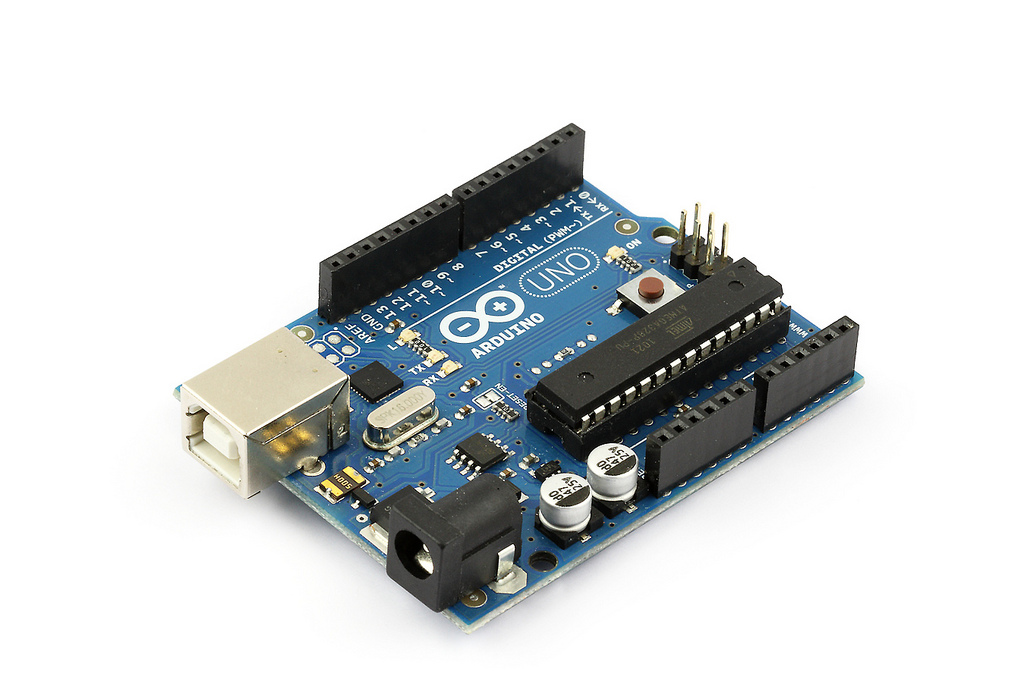
\includegraphics[width=0.5\textwidth,trim={3cm 0.5cm 3cm 3cm},clip]{images/arduino_uno.jpg}
        \caption{Arduino Uno - 16 MHz, 2 KB SRAM}
    \end{figure}
\end{frame}
\begin{frame}{Introduction}\framesubtitle{Problem Statement}
\[
\left[
\begin{minipage}{0.9\textwidth}
\centering
\begin{minipage}{0.8\textwidth}
How can a network of devices with radio transceivers of a single frequency communicate, such that any devices can send messages to other devices in the network, in a reliable while timely way?
\end{minipage}
\end{minipage}
\right]
\]
\end{frame}
\subsection{Development Process}
\begin{frame}[t]{Introduction}\framesubtitle{Development Process}
    \begin{itemize}
        \item<1-> Scrum
        \item<1-> How should we iterate?
        \item<2-> Verify new ideas and design
        \item<2-> Increasing complexity
        \item<3-> Testing hardware
            \begin{itemize}
                \item<3-> Establishing a baseline
                \item<3-> Discarding faulty devices
            \end{itemize}
        \item<4-> Test driven development?
        \begin{itemize}
            \item<4-> Difficult to test with hardware
            \item<4-> Design needs to be implemented for test
            \item<4-> Design flaws are caught late
        \end{itemize}
    \end{itemize}
\end{frame}

